
% ===========================================================================
% Title:
% ---------------------------------------------------------------------------
% to create Type I fonts type "dvips -P cmz -t letter <filename>"
% ===========================================================================
\documentclass[11pt]{article}       %--- LATEX 2e base
\usepackage{latexsym}               %--- LATEX 2e base
%---------------- Wide format -----------------------------------------------
\textwidth=6in \textheight=9in \oddsidemargin=0.25in
\evensidemargin=0.25in \topmargin=-0.5in
%--------------- Def., Theorem, Proof, etc. ---------------------------------
\newtheorem{definition}{Definition}
\newtheorem{theorem}{Theorem}
\newtheorem{lemma}{Lemma}
\newtheorem{corollary}{Corollary}
\newtheorem{property}{Property}
\newtheorem{observation}{Observation}
\newtheorem{fact}{Fact}
\newenvironment{proof}           {\noindent{\bf Proof.} }%
                                 {\null\hfill$\Box$\par\medskip}
%--------------- Algorithm --------------------------------------------------
\newtheorem{algX}{Algorithm}
\newenvironment{algorithm}       {\begin{algX}\begin{em}}%
                                 {\par\noindent --- End of Algorithm ---
                                 \end{em}\end{algX}}
\newcommand{\step}[2]            {\begin{list}{}
                                  {  \setlength{\topsep}{0cm}
                                     \setlength{\partopsep}{0cm}
                                     \setlength{\leftmargin}{0.8cm}
                                     \setlength{\labelwidth}{0.7cm}
                                     \setlength{\labelsep}{0.1cm}    }
                                  \item[#1]#2    \end{list}}
                                 % usage: \begin{algorithm} \label{xyz}
                                 %        ... \step{(1)}{...} ...
                                 %        \end{algorithm}
%--------------- Figures ----------------------------------------------------
\usepackage{graphicx}

\newcommand{\includeFig}[3]      {\begin{figure}[htb] \begin{center}
                                 \includegraphics
                                 [width=4in,keepaspectratio] %comment this line to disable scaling
                                 {#2}\caption{\label{#1}#3} \end{center} \end{figure}}
                                 % usage: \includeFig{label}{file}{caption}
%--------------- Additiona packages -----------------------------------------
\usepackage{url}
\usepackage{tikz}
\usetikzlibrary{positioning}
\tikzset{font=\scriptsize}
% ===========================================================================
\begin{document}
% ===========================================================================

% ############################################################################
% Title
% ############################################################################

\title{LITERATURE REVIEW: XRT 0.1.0 - A Language-Agnostic MapReduce Runtime for
Shared-Memory Systems}


% ############################################################################
% Author(s) (no blank lines !)
\author{
% ############################################################################
Erik Selin\\
School of Information Technology and Engineering\\
University of Ottawa\\
Ottawa, Canada K1N 6N5 \\
{\em erik.selin@gmail.com}
% ############################################################################
} % end-authors
% ############################################################################

\maketitle

% ############################################################################
\section{Introduction} \label{intro}
% ############################################################################

MapReduce is a restrictive programming model used to write efficient and highly
parallel data processing programs without having to deal with the complexities
of parallel programming. The programming model was initially introduced by
Google in 2004 \cite{GoogleMapReduce} and later popularized by Yahoo! through
the Apache open-source project Hadoop MapReduce \cite{Hadoop}. Hadoop MapReduce
provides a MapReduce runtime for networked commodity hardware and its
popularity has resulted in the development of multiple runtimes for alternative
environments like GPU’s \cite{Mars}, FGPA's \cite{Melia}, Coprocessors
\cite{MrPhi} and shared-memory systems \cite{Phoenix} \cite{Phoenix++}
\cite{CilkMR} \cite{Metis} \cite{Ostrich}.

The increasing availability of
cost-effective shared-memory systems with high core counts \cite{AWS}
\cite{GoogleCloud} means that shared-memory systems are becoming a serious
alternative to networked commodity hardware for parallel data processing.
From a previous survey of the literature it was observed that MapReduce
runtimes for shared-memory systems are all built with the sole purpose of
beating benchmarks. They tend to require the programmer to write mapper and
reducer code in C or C++, are not cross platform compatible, occasionally break
the MapReduce abstraction and in some cases are not even available for use.

The purpose of this literature review is to confirm these observations as well as
dig deeper into the literature to paint a clear picture of the current state of
MapReduce runtimes for shared-memory systems. Ultimately, the goal is to justify the
creation of XRT, a new cross-platform language-agnostic MapReduce runtime for
shared-memory systems that is inspired by Hadoop Streaming
\cite{HadoopStreaming} and based on techniques developed in modern MapReduce
runtimes for shared-memory systems \cite{Phoenix} \cite{Phoenix++} \cite{CilkMR}
\cite{Ostrich} \cite{Metis}.

% ############################################################################
\section{Literature Review} \label{litrev}
% ############################################################################

\subsection{The MapReduce programming model}

\begin{figure*}[h]
  \centering
  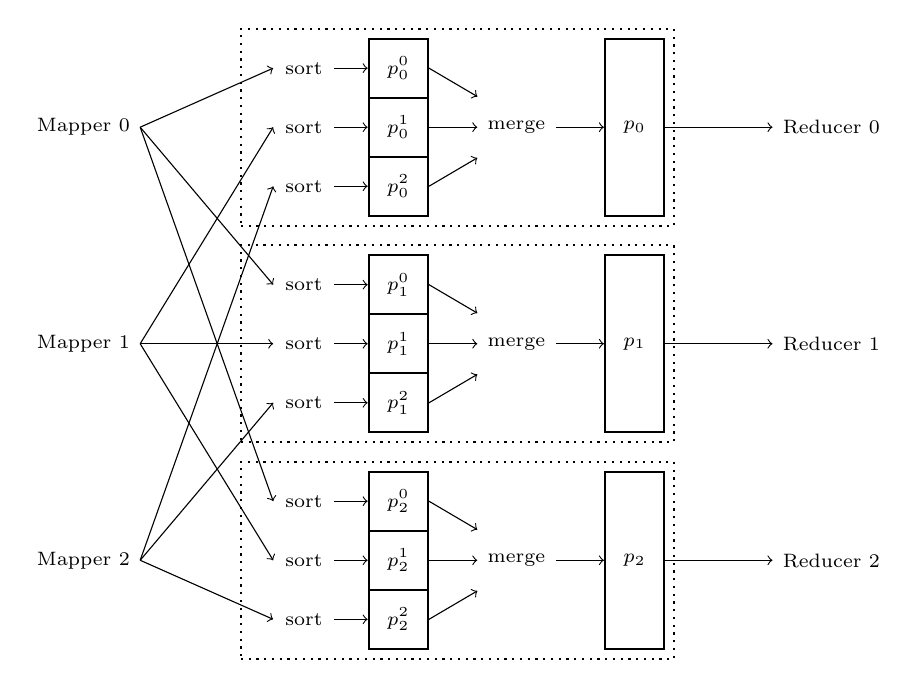
\begin{tikzpicture}[every node/.style={minimum height={0.75cm},minimum width={0.75cm},thick}]
      \node (Map2) at (0,1.25) {Mapper 2};
      \node (Map1) at (0,4) {Mapper 1};
      \node (Map0) at (0,6.75) {Mapper 0};

      \node[draw] (P20) at (4,2) { $p_2^0$ };
      \node[draw] (P21) at (4,1.25) { $p_2^1$ };
      \node[draw] (P22) at (4,0.5) { $p_2^2$ };
      \node (M2) at (5.5,1.25) {merge};
      \node (S20) at (2.8,2) {sort};
      \node (S21) at (2.8,1.25) {sort};
      \node (S22) at (2.8,0.5) {sort};
      \node[draw,minimum height={2.25cm}] (P2) at (7, 1.25) { $p_2$ };
      \node[draw,dotted,minimum height={2.5cm},minimum width={5.5cm}] at (4.75,1.25) {};

      \node[draw] (P10) at (4,4.75) { $p_1^0$ };
      \node[draw] (P11) at (4,4) { $p_1^1$ };
      \node[draw] (P12) at (4,3.25) { $p_1^2$ };
      \node (M1) at (5.5,4) {merge};
      \node (S10) at (2.8,4.75) {sort};
      \node (S11) at (2.8,4) {sort};
      \node (S12) at (2.8,3.25) {sort};
      \node[draw,minimum height={2.25cm}] (P1) at (7, 4) { $p_1$ };
      \node[draw,dotted,minimum height={2.5cm},minimum width={5.5cm}] at (4.75,4) {};

      \node[draw] (P00) at (4,7.5) { $p_0^0$ };
      \node[draw] (P01) at (4,6.75) { $p_0^1$ };
      \node[draw] (P02) at (4,6) { $p_0^2$ };
      \node (M0) at (5.5,6.75) {merge};
      \node (S00) at (2.8,7.5) {sort};
      \node (S01) at (2.8,6.75) {sort};
      \node (S02) at (2.8,6) {sort};
      \node[draw,minimum height={2.25cm}] (P0) at (7, 6.75) { $p_0$ };
      \node[draw,dotted,minimum height={2.5cm},minimum width={5.5cm}] at (4.75,6.75) {};

      \node (R2) at (9.5,1.25) {Reducer 2};
      \node (R1) at (9.5,4) {Reducer 1};
      \node (R0) at (9.5,6.75) {Reducer 0};

      \path [->](Map0.east) edge node {} (S00.west);
      \path [->](Map0.east) edge node {} (S10.west);
      \path [->](Map0.east) edge node {} (S20.west);
      \path [->](Map1.east) edge node {} (S01.west);
      \path [->](Map1.east) edge node {} (S11.west);
      \path [->](Map1.east) edge node {} (S21.west);
      \path [->](Map2.east) edge node {} (S02.west);
      \path [->](Map2.east) edge node {} (S12.west);
      \path [->](Map2.east) edge node {} (S22.west);

      \path [->](S00.east) edge node {} (P00.west);
      \path [->](S10.east) edge node {} (P10.west);
      \path [->](S20.east) edge node {} (P20.west);
      \path [->](S01.east) edge node {} (P01.west);
      \path [->](S11.east) edge node {} (P11.west);
      \path [->](S21.east) edge node {} (P21.west);
      \path [->](S02.east) edge node {} (P02.west);
      \path [->](S12.east) edge node {} (P12.west);
      \path [->](S22.east) edge node {} (P22.west);

      \path [->](P00.east) edge node {} (M0.north west);
      \path [->](P01.east) edge node {} (M0.west);
      \path [->](P02.east) edge node {} (M0.south west);
      \path [->](P10.east) edge node {} (M1.north west);
      \path [->](P11.east) edge node {} (M1.west);
      \path [->](P12.east) edge node {} (M1.south west);
      \path [->](P20.east) edge node {} (M2.north west);
      \path [->](P21.east) edge node {} (M2.west);
      \path [->](P22.east) edge node {} (M2.south west);

      \path [->](M0.east) edge node {} (P0.west);
      \path [->](M1.east) edge node {} (P1.west);
      \path [->](M2.east) edge node {} (P2.west);

      \path [->](P0.east) edge node {} (R0.west);
      \path [->](P1.east) edge node {} (R1.west);
      \path [->](P2.east) edge node {} (R2.west);
  \end{tikzpicture}
  \caption{Classical MapReduce programming model.}
  \label{fig:mapreduce}
\end{figure*}


In the classical MapReduce programming model \cite{GoogleMapReduce}, illustrated in
Figure \ref{fig:mapreduce}, programmers only need to supply mapper
and reducer programs together with the source of the input and the destination
of the output, everything else is handled by the runtime. For most MapReduce
runtimes this means executing parallel workers running multiple instances of the
mapper and reducer programs, reading and distribution of the input, collection
and writing of the output and shuffling and sorting intermediate data. A
classical MapReduce job starts by splitting the input and running a mapper for
each split. Each mapper will consume the records in the split and output
key-value pairs which are collected by the runtime and partitioned into sorted
buckets. Key-value pairs with the same key end up in the same bucket no
matter which mapper produced the pair. Once all mappers are done a reducer is
started for each bucket and all key-value pairs in the bucket are processed in
order. This means that all key-value pairs produced
by the mappers with the same key will all be processed by the same reducer. Finally,
the output of the reducers becomes the output of the job.

There is a lot of room
for implementation specific deviations and optimizations in this description but on
a high level all MapReduce runtimes operates by this model \cite{GoogleMapReduce}
\cite{Hadoop} \cite{Phoenix} \cite{Phoenix++} \cite{CilkMR} \cite{Metis}
\cite{Ostrich}. The success of the MapReduce model comes from the ease of writing
sequential mapper and reducer programs that are able to accomplish advanced
data transformation tasks in parallel when executed through a MapReduce runtime
\cite{GoogleMapReduce}.

\subsection{MapReduce language support}

MapReduce runtimes with multi-language or language-agnostic support is not something that has been greatly explored by the MapReduce community.
In general MapReduce runtimes are single language: Googles proprietary MapReduce is described as a C++ runtime \cite{GoogleMapReduce}, Hadoop MapReduce provides a runtime for Java \cite{Hadoop} and shared-memory runtimes like Phoenix \cite{Phoenix},
Phoenix++ \cite{Phoenix++}, Metis \cite{Metis}, Ostrich \cite{Ostrich} and
CilkMR \cite{CilkMR} provide runtimes for C or C++.

In fact, the only available language-agnostic MapReduce runtime seems to be Hadoop Streaming.
Hadoop Streaming is built upon Hadoop MapReduce and achieves language-agnostic support by replacing the mappers and reducers with externally run processes that communicates with the MapReduce runtime over the standard streams \cite{HadoopStreaming}.
Unfortunately the MapReduce runtime that power Hadoop Streaming is still the Java optimized Hadoop MapReduce runtime and the resulting performance of Hadoop Streaming is very bad \cite{HadoopStreamingPerf} \cite{Pydoop} \cite{Perldoop}.
ShmStreaming is an attempt to increase the performance of Hadoop Streaming by communicating over shared memory instead of the standard streams \cite{ShmStreaming}.
The performance of Hadoop Streaming + ShmStreaming is superior to Hadoop Streaming but communication over shared memory is not as straightforward to implement compared to communication over standard streams.
In addition, ShmStreaming still suffers from the fact that Hadoop MapReduce is not optimized for interacting with mappers and reducers that are run as external processes.

The Hadoop community has also developed Hadoop Pipes which outperforms Hadoop Streaming but only offers support for C++ \cite{HadoopPipes}.
Language support for the python programming language without using Hadoop Streaming is available through the Pydoop project.
Pydoop integrates with Hadoop MapReduce by wrapping Hadoop Pipes and offers superior performance versus running python mapper and reducers through Hadoop Streaming \cite{Pydoop}.
An alternative approach to adding specific language support to Hadoop MapReduce was undertaken in the Perldoop project \cite{Perldoop}.
Perldoop provides a perl-to-java transpiler specifically built to convert Perl Hadoop MapReduce jobs to Java Hadoop MapReduce jobs.
Perldoop can achieve very good performance since it is effectively running regular Java Hadoop MapReduce however there are a lot of limitations since only a subset of very specifically formatted Perl is supported.

Finally, there seems to be no MapReduce runtime that is built explicitly for multi-language or truly language-agnostic MapReduce.

\subsection{MapReduce on shared-memory systems}

Shared-memory systems are becoming increasingly capable and cost effective for
data processing. At the time of writing it is possible to get a on demand
system with 128 cores and 3.9 terabytes of memory for \$26/hour \cite{AWS}.
Based on recent releases from popular cloud providers the trend of affordable
high core-count systems is likely to continue and cost per core will likely
keep decreasing \cite{AWS} \cite{GoogleCloud}.

\begin{figure}[h]
  \centering
  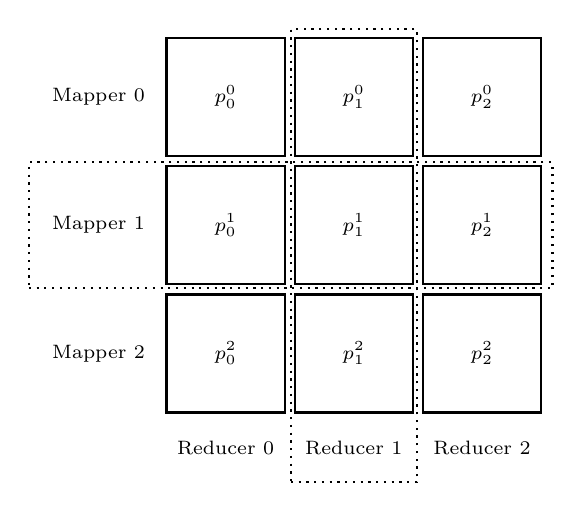
\begin{tikzpicture}[every node/.style={minimum height={1.5cm},minimum width={1.5cm},thick}]
    \matrix[row sep=1mm, column sep=1mm] (m)
    {
      \node { Mapper 0 }; & \node[draw] { $p_0^0$ }; & \node[draw] (c1) { $p_1^0$ }; & \node[draw] { $p_2^0$}; \\
      \node (r1) { Mapper 1 }; & \node[draw] { $p_0^1$ }; & \node[draw] { $p_1^1$ }; & \node[draw] { $p_2^1$ }; \\
      \node { Mapper 2 }; & \node[draw] (node0) { $p_0^2$}; & \node[draw] (node1) { $p_1^2$ }; & \node[draw] (node2) { $p_2^2$ }; \\
    };

    \node[below=1.75cm of node0.north,minimum height=0cm] {Reducer 0};
    \node[below=1.75cm of node1.north,minimum height=0cm] {Reducer 1};
    \node[below=1.75cm of node2.north,minimum height=0cm] {Reducer 2};

    \node[below=-1.1mm of c1.north,draw,dotted,minimum height=5.75cm,minimum width=1.6cm] {};
    \node[below right=-0.5mm and -0.9cm of r1.north,draw,dotted,minimum height=1.6cm,minimum width=6.65cm] {};
  \end{tikzpicture}
  \caption{Memory layout in shared-memory MapReduce runtimes.}
  \label{fig:memorylayout}
\end{figure}


MapReduce on shared-memory systems was first explored by the Phoenix \cite{Phoenix} project.
Besides being first to explore MapReduce on shared-memory systems the Phoenix project also contributed the matrix memory-layout illustrated in Figure \ref{fig:memorylayout}.
This memory layout is used in some form by all shared-memory runtimes \cite{Phoenix} \cite{Phoenix++} \cite{CilkMR} \cite{Metis} \cite{Ostrich} and enables workers to communicate
extremely efficiently with the runtime while avoiding contention.
The columns in the matrix represent partitions and each entry in the matrix is a buffer responsible for storing the intermediate data produced by a mapper.
During the mapper stage each mapper is given access to a row in the matrix and during the reducer stage each reducer is given access to a column in the matrix.
This methodology ensures that no communication is required across workers during execution which in turns maximizes throughput.

The Phoenix runtime has gone through multiple iterations and Phoenix 2.0 was the result of performance issues when Phoenix was run on larger shared-memory systems processing larger data sets \cite{Phoenix2}.
In particular the intermediate data buffers that are used to store keys from the key-value pairs produced by the mappers are implemented as sorted arrays in Phoenix.
This lead to performance issues since the arrays needed to reallocate whenever they ran out of space and whenever a new key was added all keys coming after the new key had to be shifted.
Phoenix 2.0 solved this issue by significantly increasing the number of sorted key arrays so that on average only one key resides in each array \cite{Phoenix2}.

Further work on the Phoenix project has lead to the determination that the intermediate sorted arrays were limiting the potential performance of the runtime.
This resulted in the reimplementation of Phoenix in C++ and the start of the Phoenix++ project \cite{Phoenix++}.
Phoenix++ is the poster child of shared-memory MapReduce runtimes optimized for speed and extends the MapReduce API to include containers and combiner objects.
Containers exposes the internals of the shuffle stage to the programmer and makes it possible to select or tune the data structure used for shuffling \cite{Phoenix++}.
Combiner objects exposes the internals of the intermediate data buffers and makes it possible to select the data structure used for intermediate data buffering \cite{Phoenix++}.
While the introduction of containers and combiner objects in Phoenix++ does allow for better performance it has been argued that they break the MapReduce abstraction and programmers now need to be intimately familiar with the Phoenix++ internals to pick the correct containers and combiner objects \cite{CilkMR}.

An alternative approach to dealing with the perceived shortcomings of the Phoenix project is the Metis project.
Instead of increasing the configurability of the runtime Metis introduces a compromise intermediate data buffer \cite{Metis}.
Using a more advanced buffer Metis is able to achieve significant performance increase over Phoenix on data processing problems involving very little mapper/reducer computation on datasets with few keys but many duplicates.
Metis does not offer any performance increase over Phoenix on data processing jobs involving a significant amount of mapper/reducer computation or on datasets with few duplicate keys \cite{Metis}.

An extension of the Phoenix model is Tiled-MapReduce and its prototype implementation Ostrich.
Ostrich extends the model introduced by Phoenix by using the tiling strategy commonly used in the compiler community.
Ostrich and Tiled-MapReduce runs splits the input into subsets and runs smaller jobs on each subset.
Each smaller job runs mappers that produces a intermediate data buffer like Phoenix but then reduces the partial intermediate data buffer using a combiner into a secondary intermediate data buffer.
Once all smaller jobs have run the secondary intermediate data buffers are reduced by the reducers.
Since the combiner reduces the amount of intermediate data this approach increases the performance of the runtime and allows for processing of more data.
In addition the primary intermediate data buffer that is filled by the mappers can be reused between the smaller jobs.
This means that Ostrich is able to avoid a lot of memory allocation calls compared to Phoenix and other shared-memory runtimes \cite{Ostrich}.

The CilkMR project is one of the newest MapReduce runtimes for shared-memory systems and addresses the key-value pair serialization/deserialization overhead of all the previously discussed runtimes \cite{CilkMR}.
Instead of operating on key-value pairs CilkMR operates over typed data containers which means that the mappers can pass arbitrary data structures to the reducers.
CilkMR is also inspired by Phoenix++ in that it allows the programmers to control intermediate data structures and tune the runtime.
The performance of CilkMR is really good on computationally heavy tasks since mappers and reducers can operate on complex data structures.
However, Phoenix++ performs better than CilkMR on classical data processing jobs like wc and strmatch \cite{CilkMR} \cite{GoogleMapReduce}.

A completely different idea for bringing MapReduce to shared-memory systems is the Hone project.
Hone attempts to take advantage of the familiarity of Hadoop MapReduce by providing a Hadoop MapReduce compatible Java API \cite{ScalingDown}.
The goal is to create a a runtime that allow you to run the exact same Java code that was written for Hadoop MapReduce.
In benchmarks Hone beats Phoenix however Phoenix++ beats Phoenix by a much wider margin and thus it seems like Phoenix++ is likely much faster then Hone.

A last note about recent development in shared-memory MapReduce runtimes is the usage of disk based data structures.
In Hadoop MapReduce almost all intermediate data will reside on disk at some point but in all the above mentioned shared-memory runtimes there is never a mention of disk backing.
There has been some exploration in extending Metis to include the capacity of spilling intermediate data to disk if the input is too large \cite{DiskOptimization}.
However, this optimization was never contributed back to the Metis project.

% ############################################################################
\section{Conclusion} \label{conclusion}
% ############################################################################

The field of shared-memory MapReduce runtimes is still extremely young and
almost all efforts are focused on beating benchmarks. Programming mapper and
reducer code for shared-memory MapReduce runtimes requires knowledge of C or C++
and sometimes a deep understanding of the runtime internals. A surprising
discovery from this review is that the shared-memory MapReduce community is not
really considering handling data that is too large to fit in memory.

Following the literature review the case for building XRT has been strengthen.
Shared-memory MapReduce runtimes lack a cross platform, disk aware and simple to
use runtime and the broader MapReduce community lack exploration of language
agnostic runtimes. That being said a lot of great ideas have already been
developed by the shared-memory MapReduce runtimes. Concepts like the matrix
memory layout, intermediate data structure reuse and language-agnostic support
through communication over standard streams will all be brough into XRT.

% ############################################################################
% Bibliography
% ############################################################################
\bibliographystyle{plain}
\bibliography{bibliography}     %loads bibliography.bib

% ============================================================================
\end{document}
% ============================================================================
